% AUTO-GENERATED by scripts/make_confirm2_appendix.py -- floats of Appendix C (captions: drafts for David).
% Not input by main.tex; intended to replace the placeholder paragraph of app:confirm2.

\begin{figure*}[!t]
\centering
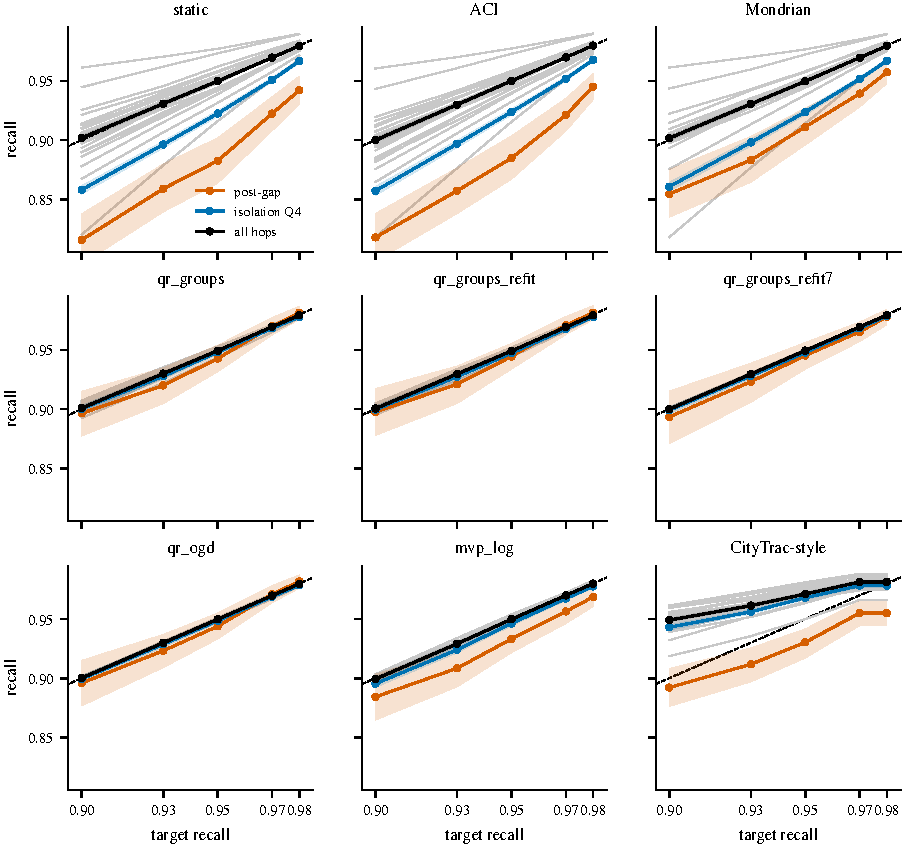
\includegraphics[width=\textwidth]{generated/figures/fig_c2_calibration_block1.pdf}
\caption{Recall per group against the target, block~1 (August); as Fig.~\ref{fig:c2_calibration}.}
\label{fig:c2_calibration_block1}
\end{figure*}

\begin{figure*}[!t]
\centering
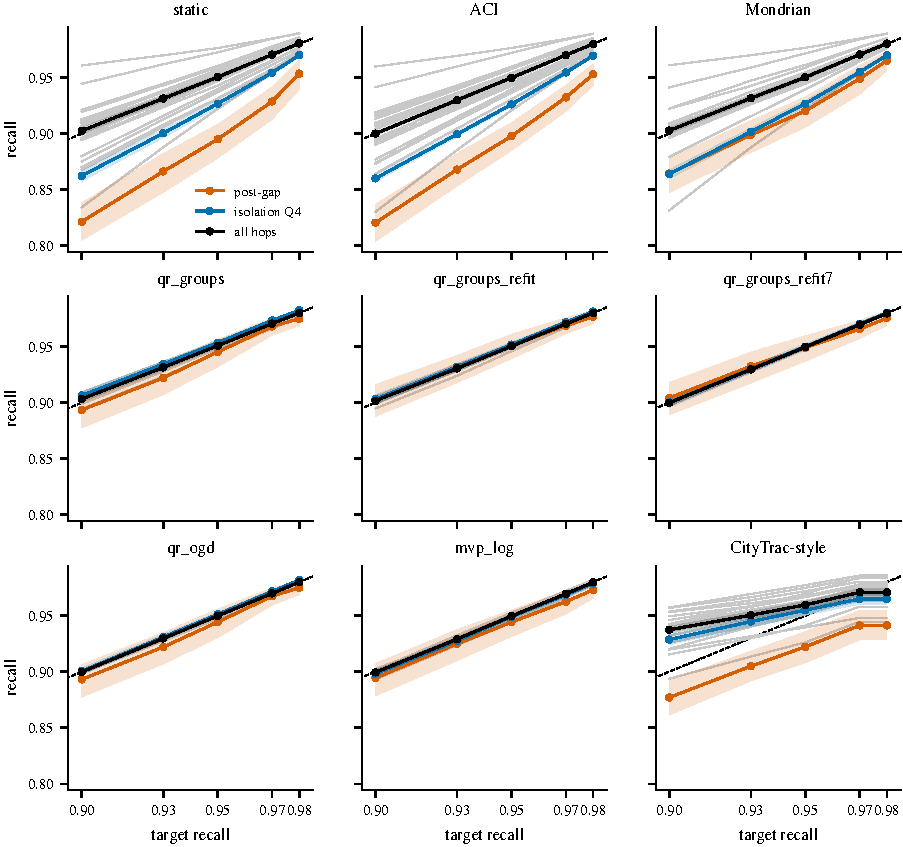
\includegraphics[width=\textwidth]{generated/figures/fig_c2_calibration_block2.pdf}
\caption{Recall per group against the target, block~2 (autumn); as Fig.~\ref{fig:c2_calibration}.}
\label{fig:c2_calibration_block2}
\end{figure*}

\begin{figure*}[!t]
\centering
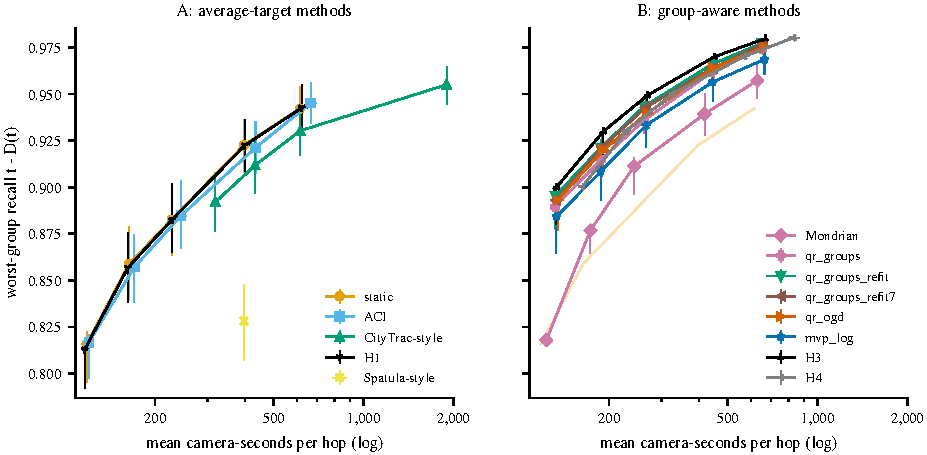
\includegraphics[width=\textwidth]{generated/figures/fig_c2_cost_block1.pdf}
\caption{Worst-group recall against mean cost per hop, block~1; as Fig.~\ref{fig:c2_cost}.}
\label{fig:c2_cost_block1}
\end{figure*}

\begin{figure*}[!t]
\centering
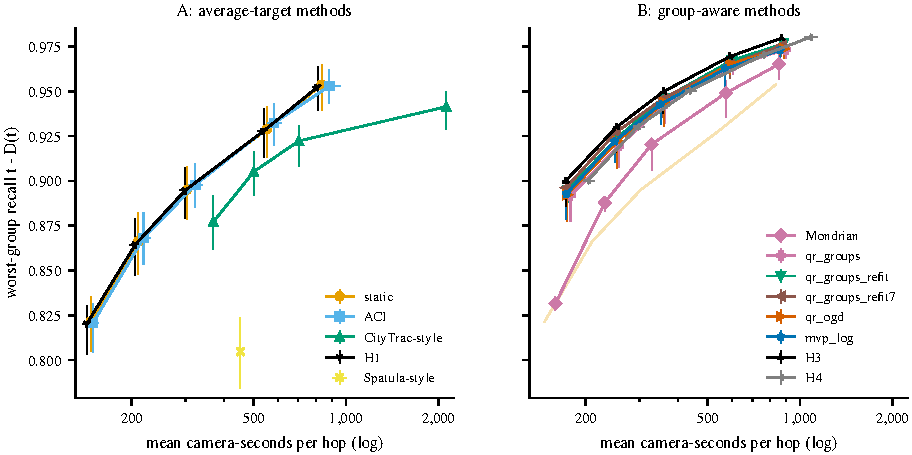
\includegraphics[width=\textwidth]{generated/figures/fig_c2_cost_block2.pdf}
\caption{Worst-group recall against mean cost per hop, block~2; as Fig.~\ref{fig:c2_cost}.}
\label{fig:c2_cost_block2}
\end{figure*}

\begin{table*}[!t]
\centering
\caption{Confirmation period, target 0.90; columns as in Table~\ref{tab:c2_main}.}
\label{tab:c2_app_t0900}
\footnotesize
% source: results/porto_cctv_confirm2/analysis/deficits.csv @ 1a806b3; results/porto_cctv_confirm2/analysis/costs.csv @ 1a806b3; results/porto_cctv_confirm2/analysis/cost_ratios.csv @ 1a806b3; results/porto_cctv_confirm2/analysis/method_points.csv @ 1a806b3; results/porto_cctv_confirm2/analysis/hindsight.csv @ 1a806b3; results/porto_cctv_confirm2/analysis/seed_range.csv @ 1a806b3; exploratory/ref_group_d/ref_group_d.csv @ f484865
% scope=combined (56 days), target=0.9, seed means; d and Dbar in pp with conservative 95% intervals (deficits.csv cells hopkind=2, nn_bin=3, WORST: deficit [lo, hi]; H rows: Dbar = t - worst_recall of method_points.csv with [t - worst_hi, t - worst_lo]); recall = recall_all (costs.csv) or hindsight.csv; cost = cost_mean (camera-seconds per hop); ratios = cost_ratios.csv ratio (H3: threshold fixed); seeds = D_seed_min-D_seed_max of seed_range.csv (pp; one value for seed-independent methods).
\setlength{\tabcolsep}{4.5pt}
\begin{tabular}{@{}lrrrrrrrrrr@{}}
\toprule
 & \multicolumn{3}{c}{Shortfall (pp), 95\% interval} & & & & \multicolumn{4}{c}{Cost ratio to} \\
\cmidrule(lr){2-4}\cmidrule(l){8-11}
Method & Post-gap $d$ & Isolation Q4 $d$ & \Dbar{} & $D^s$, seeds & Recall & Cost & H1 & H2 & H3 & H4 \\
\midrule
\texttt{mvp\_log} & 1.0 [$-$0.1, 2.1] & 0.3 [0.1, 0.5] & 1.0 [0.5, 2.1] & 0.8--1.3 & 0.899 & 155 & 1.18 & 1.19 & 1.00 & 0.84 \\
\texttt{qr\_ogd} & 0.6 [$-$0.5, 1.8] & $-$0.0 [$-$0.2, 0.2] & 0.7 [0.2, 1.8] & 0.2--1.4 & 0.900 & 157 & 1.19 & 1.19 & 1.01 & 0.85 \\
\addlinespace
\texttt{static} & 8.1 [6.8, 9.5] & 3.9 [3.7, 4.2] & 8.1 [7.1, 9.5] & 8.1 & 0.902 & 134 & 1.02 & 1.00 & 0.87 & 0.73 \\
ACI & 8.1 [6.8, 9.4] & 4.1 [3.8, 4.4] & 8.1 [7.4, 9.4] & 7.8--8.2 & 0.900 & 136 & 1.04 & 1.04 & 0.88 & 0.74 \\
Mondrian & 4.0 [2.8, 5.2] & 3.7 [3.5, 4.0] & 7.4 [7.2, 7.7] & 7.4 & 0.902 & 143 & 1.09 & 1.07 & 0.93 & 0.77 \\
\texttt{qr\_groups} & 0.5 [$-$0.5, 1.7] & $-$0.4 [$-$0.6, $-$0.1] & 0.8 [0.3, 1.7] & 0.4--1.3 & 0.902 & 158 & 1.20 & 1.17 & 1.02 & 0.85 \\
\texttt{qr\_groups\_refit} & $-$0.1 [$-$1.2, 1.1] & $-$0.2 [$-$0.4, 0.1] & 0.3 [0.1, 1.1] & 0.2--0.3 & 0.901 & 156 & 1.19 & 1.17 & 1.01 & 0.84 \\
\texttt{qr\_groups\_refit7} & 0.0 [$-$1.2, 1.2] & 0.0 [$-$0.2, 0.3] & 0.3 [0.1, 1.2] & 0.1--0.8 & 0.900 & 155 & 1.18 & 1.18 & 1.00 & 0.84 \\
CityTrac-style & 1.7 [0.6, 2.8] & $-$3.5 [$-$3.7, $-$3.2] & 1.7 [0.6, 2.8] & 1.7 & 0.943 & 347 & 2.65 & 1.52 & 2.24 & 1.88 \\
Spatula-style & 8.6 [7.1, 10.1] & 1.7 [1.4, 2.1] & 8.6 [7.1, 10.1] & 8.6 & 0.909 & 428 & 3.27 & 2.98 & 2.77 & 2.31 \\
\addlinespace
H1 & 8.3$^\dagger$ & 4.2$^\dagger$ & 8.3 [7.5, 9.7] & & 0.900 & 131 &  &  &  & \\
H2$^{a}$ & n/a & n/a & n/a & & 0.899--0.943 & 130--229 &  &  &  & \\
H3 & 0.0$^\dagger$ & 0.0$^\dagger$ & 0.0 [$-$0.0, 1.2] & & 0.900 & 155 &  &  &  & \\
H4 & $-$0.0$^\dagger$ & $-$0.6$^\dagger$ & $-$0.0 [$-$0.0, $-$0.0] & & 0.930 & 185 &  &  &  & \\
\bottomrule
\end{tabular}

\smallskip\parbox{\textwidth}{\footnotesize $^{a}$H2 is fitted to each method's overall recall (per seed); the row gives the range over the ten methods of the seed-mean recall and cost. $^\dagger$Additional analysis; point estimate, no interval. n/a: not computed.}

\end{table*}

\begin{table*}[!t]
\centering
\caption{Confirmation period, target 0.93; columns as in Table~\ref{tab:c2_main}.}
\label{tab:c2_app_t0930}
\footnotesize
% source: results/porto_cctv_confirm2/analysis/deficits.csv @ 1a806b3; results/porto_cctv_confirm2/analysis/costs.csv @ 1a806b3; results/porto_cctv_confirm2/analysis/cost_ratios.csv @ 1a806b3; results/porto_cctv_confirm2/analysis/method_points.csv @ 1a806b3; results/porto_cctv_confirm2/analysis/hindsight.csv @ 1a806b3; results/porto_cctv_confirm2/analysis/seed_range.csv @ 1a806b3; exploratory/ref_group_d/ref_group_d.csv @ f484865
% scope=combined (56 days), target=0.93, seed means; d and Dbar in pp with conservative 95% intervals (deficits.csv cells hopkind=2, nn_bin=3, WORST: deficit [lo, hi]; H rows: Dbar = t - worst_recall of method_points.csv with [t - worst_hi, t - worst_lo]); recall = recall_all (costs.csv) or hindsight.csv; cost = cost_mean (camera-seconds per hop); ratios = cost_ratios.csv ratio (H3: threshold fixed); seeds = D_seed_min-D_seed_max of seed_range.csv (pp; one value for seed-independent methods).
\setlength{\tabcolsep}{4.5pt}
\begin{tabular}{@{}lrrrrrrrrrr@{}}
\toprule
 & \multicolumn{3}{c}{Shortfall (pp), 95\% interval} & & & & \multicolumn{4}{c}{Cost ratio to} \\
\cmidrule(lr){2-4}\cmidrule(l){8-11}
Method & Post-gap $d$ & Isolation Q4 $d$ & \Dbar{} & $D^s$, seeds & Recall & Cost & H1 & H2 & H3 & H4 \\
\midrule
\texttt{mvp\_log} & 1.2 [0.2, 2.3] & 0.4 [0.2, 0.6] & 1.2 [0.6, 2.3] & 0.8--1.7 & 0.929 & 222 & 1.19 & 1.20 & 0.98 & 0.83 \\
\texttt{qr\_ogd} & 0.7 [$-$0.2, 1.8] & 0.0 [$-$0.2, 0.2] & 0.9 [0.3, 1.9] & 0.2--1.5 & 0.930 & 226 & 1.21 & 1.22 & 1.00 & 0.85 \\
\addlinespace
\texttt{static} & 6.7 [5.4, 8.0] & 3.1 [2.9, 3.4] & 6.7 [5.4, 8.0] & 6.7 & 0.931 & 190 & 1.02 & 1.00 & 0.84 & 0.71 \\
ACI & 6.6 [5.5, 7.8] & 3.2 [2.9, 3.4] & 6.6 [5.5, 7.8] & 6.4--6.8 & 0.930 & 197 & 1.06 & 1.06 & 0.88 & 0.74 \\
Mondrian & 3.8 [2.7, 4.9] & 3.0 [2.8, 3.2] & 4.7 [4.5, 5.0] & 4.7 & 0.931 & 205 & 1.10 & 1.08 & 0.91 & 0.77 \\
\texttt{qr\_groups} & 0.9 [$-$0.1, 2.0] & $-$0.2 [$-$0.3, 0.0] & 1.1 [0.5, 2.0] & 0.4--1.7 & 0.931 & 226 & 1.21 & 1.19 & 1.01 & 0.85 \\
\texttt{qr\_groups\_refit} & 0.3 [$-$0.6, 1.3] & 0.0 [$-$0.2, 0.2] & 0.4 [0.2, 1.3] & 0.3--0.5 & 0.930 & 224 & 1.20 & 1.20 & 1.00 & 0.84 \\
\texttt{qr\_groups\_refit7} & 0.1 [$-$0.9, 1.2] & 0.1 [$-$0.1, 0.3] & 0.3 [0.1, 1.3] & 0.1--0.6 & 0.930 & 224 & 1.20 & 1.21 & 1.00 & 0.84 \\
CityTrac-style & 2.2 [1.3, 3.2] & $-$2.0 [$-$2.2, $-$1.7] & 2.2 [1.3, 3.2] & 2.2 & 0.955 & 470 & 2.52 & 1.55 & 2.09 & 1.77 \\
Spatula-style & 11.6 [10.1, 13.1] & 4.7 [4.4, 5.1] & 11.6 [10.1, 13.1] & 11.6 & 0.909 & 428 & 2.30 & 2.98 & 1.90 & 1.61 \\
\addlinespace
H1 & 6.9$^\dagger$ & 3.3$^\dagger$ & 6.9 [5.7, 8.1] & & 0.930 & 186 &  &  &  & \\
H2$^{a}$ & --- & --- & --- & & 0.909--0.955 & 144--304 &  &  &  & \\
H3 & 0.0$^\dagger$ & 0.0$^\dagger$ & 0.0 [0.0, 1.0] & & 0.930 & 225 &  &  &  & \\
H4 & 0.0$^\dagger$ & $-$0.2$^\dagger$ & 0.0 [0.0, 0.0] & & 0.950 & 266 &  &  &  & \\
\bottomrule
\end{tabular}

\smallskip\parbox{\textwidth}{\footnotesize $^{a}$H2 is fitted to each method's overall recall (per seed), so it has no shortfall of its own; the row gives the range over the ten methods of the seed-mean recall and cost. $^\dagger$Additional analysis; point estimate, no interval.}

\end{table*}

\begin{table*}[!t]
\centering
\caption{Confirmation period, target 0.97; columns as in Table~\ref{tab:c2_main}.}
\label{tab:c2_app_t0970}
\footnotesize
% source: results/porto_cctv_confirm2/analysis/deficits.csv @ 1a806b3; results/porto_cctv_confirm2/analysis/costs.csv @ 1a806b3; results/porto_cctv_confirm2/analysis/cost_ratios.csv @ 1a806b3; results/porto_cctv_confirm2/analysis/method_points.csv @ 1a806b3; results/porto_cctv_confirm2/analysis/hindsight.csv @ 1a806b3; results/porto_cctv_confirm2/analysis/seed_range.csv @ 1a806b3; exploratory/ref_group_d/ref_group_d.csv @ f484865
% scope=combined (56 days), target=0.97, seed means; d and Dbar in pp with conservative 95% intervals (deficits.csv cells hopkind=2, nn_bin=3, WORST: deficit [lo, hi]; H rows: Dbar = t - worst_recall of method_points.csv with [t - worst_hi, t - worst_lo]); recall = recall_all (costs.csv) or hindsight.csv; cost = cost_mean (camera-seconds per hop); ratios = cost_ratios.csv ratio (H3: threshold fixed); seeds = D_seed_min-D_seed_max of seed_range.csv (pp; one value for seed-independent methods).
\setlength{\tabcolsep}{4.5pt}
\begin{tabular}{@{}lrrrrrrrrrr@{}}
\toprule
 & \multicolumn{3}{c}{Shortfall (pp), 95\% interval} & & & & \multicolumn{4}{c}{Cost ratio to} \\
\cmidrule(lr){2-4}\cmidrule(l){8-11}
Method & Post-gap $d$ & Isolation Q4 $d$ & \Dbar{} & $D^s$, seeds & Recall & Cost & H1 & H2 & H3 & H4 \\
\midrule
\texttt{mvp\_log} & 1.0 [0.3, 1.7] & 0.2 [0.1, 0.3] & 1.0 [0.4, 1.7] & 0.7--1.2 & 0.970 & 515 & 1.08 & 1.09 & 0.98 & 0.76 \\
\texttt{qr\_ogd} & 0.1 [$-$0.4, 0.7] & $-$0.1 [$-$0.2, 0.0] & 0.4 [0.2, 0.7] & 0.1--1.1 & 0.970 & 529 & 1.11 & 1.11 & 1.00 & 0.78 \\
\addlinespace
\texttt{static} & 4.4 [3.4, 5.5] & 1.7 [1.6, 1.8] & 4.4 [3.4, 5.5] & 4.4 & 0.970 & 483 & 1.01 & 1.00 & 0.91 & 0.72 \\
ACI & 4.2 [3.4, 5.2] & 1.7 [1.5, 1.8] & 4.2 [3.4, 5.2] & 4.2--4.3 & 0.970 & 517 & 1.08 & 1.08 & 0.98 & 0.77 \\
Mondrian & 2.5 [1.7, 3.4] & 1.6 [1.5, 1.8] & 2.5 [1.7, 3.4] & 2.5 & 0.970 & 505 & 1.06 & 1.04 & 0.96 & 0.75 \\
\texttt{qr\_groups} & 0.1 [$-$0.4, 0.6] & $-$0.1 [$-$0.2, $-$0.0] & 0.4 [0.3, 0.8] & 0.2--1.2 & 0.970 & 534 & 1.12 & 1.11 & 1.01 & 0.79 \\
\texttt{qr\_groups\_refit} & 0.0 [$-$0.5, 0.6] & $-$0.0 [$-$0.1, 0.1] & 0.2 [0.1, 0.6] & 0.1--0.3 & 0.970 & 530 & 1.11 & 1.11 & 1.00 & 0.79 \\
\texttt{qr\_groups\_refit7} & 0.4 [$-$0.1, 1.0] & 0.0 [$-$0.1, 0.2] & 0.5 [0.2, 1.1] & 0.1--0.8 & 0.970 & 526 & 1.10 & 1.12 & 1.00 & 0.78 \\
CityTrac-style & 2.3 [1.4, 3.2] & $-$0.1 [$-$0.3, 0.2] & 2.3 [1.5, 3.2] & 2.3 & 0.976 & 2025 & 4.24 & 3.34 & 3.83 & 3.01 \\
Spatula-style & 15.6 [14.1, 17.1] & 8.7 [8.4, 9.1] & 15.6 [14.1, 17.1] & 15.6 & 0.909 & 428 & 0.90 & 2.98 & 0.81 & 0.64 \\
\addlinespace
H1 & 4.4$^\dagger$ & 1.7$^\dagger$ & 4.4 [3.5, 5.5] & & 0.970 & 478 &  &  &  & \\
H2$^{a}$ & n/a & n/a & n/a & & 0.909--0.976 & 144--607 &  &  &  & \\
H3 & 0.0$^\dagger$ & $-$0.0$^\dagger$ & 0.0 [0.0, 0.6] & & 0.970 & 528 &  &  &  & \\
H4 & $-$0.0$^\dagger$ & $-$0.0$^\dagger$ & $-$0.0 [$-$0.0, $-$0.0] & & 0.979 & 674 &  &  &  & \\
\bottomrule
\end{tabular}

\smallskip\parbox{\textwidth}{\footnotesize $^{a}$H2 is fitted to each method's overall recall (per seed); the row gives the range over the ten methods of the seed-mean recall and cost. $^\dagger$Additional analysis; point estimate, no interval. n/a: not computed.}

\end{table*}

\begin{table*}[!t]
\centering
\caption{Confirmation period, target 0.98; columns as in Table~\ref{tab:c2_main}.}
\label{tab:c2_app_t0980}
\footnotesize
% source: results/porto_cctv_confirm2/analysis/deficits.csv @ 1a806b3; results/porto_cctv_confirm2/analysis/costs.csv @ 1a806b3; results/porto_cctv_confirm2/analysis/cost_ratios.csv @ 1a806b3; results/porto_cctv_confirm2/analysis/method_points.csv @ 1a806b3; results/porto_cctv_confirm2/analysis/hindsight.csv @ 1a806b3; results/porto_cctv_confirm2/analysis/seed_range.csv @ 1a806b3; exploratory/ref_group_d/ref_group_d.csv @ f484865
% scope=combined (56 days), target=0.98, seed means; d and Dbar in pp with conservative 95% intervals (deficits.csv cells hopkind=2, nn_bin=3, WORST: deficit [lo, hi]; H rows: Dbar = t - worst_recall of method_points.csv with [t - worst_hi, t - worst_lo]); recall = recall_all (costs.csv) or hindsight.csv; cost = cost_mean (camera-seconds per hop); ratios = cost_ratios.csv ratio (H3: threshold fixed); seeds = D_seed_min-D_seed_max of seed_range.csv (pp; one value for seed-independent methods).
\setlength{\tabcolsep}{4.5pt}
\begin{tabular}{@{}lrrrrrrrrrr@{}}
\toprule
 & \multicolumn{3}{c}{Shortfall (pp), 95\% interval} & & & & \multicolumn{4}{c}{Cost ratio to} \\
\cmidrule(lr){2-4}\cmidrule(l){8-11}
Method & Post-gap $d$ & Isolation Q4 $d$ & \Dbar{} & $D^s$, seeds & Recall & Cost & H1 & H2 & H3 & H4 \\
\midrule
\texttt{mvp\_log} & 0.9 [0.3, 1.4] & 0.2 [0.1, 0.3] & 0.9 [0.4, 1.4] & 0.6--1.1 & 0.980 & 773 & 1.07 & 1.07 & 0.99 & 0.80 \\
\texttt{qr\_ogd} & 0.2 [$-$0.2, 0.7] & $-$0.0 [$-$0.1, 0.0] & 0.4 [0.2, 0.8] & 0.1--1.0 & 0.980 & 787 & 1.08 & 1.09 & 1.01 & 0.81 \\
\addlinespace
\texttt{static} & 3.1 [2.3, 4.0] & 1.1 [1.0, 1.2] & 3.1 [2.3, 4.0] & 3.1 & 0.980 & 735 & 1.01 & 1.00 & 0.94 & 0.76 \\
ACI & 3.0 [2.3, 3.7] & 1.1 [1.0, 1.2] & 3.0 [2.3, 3.7] & 2.9--3.1 & 0.980 & 786 & 1.08 & 1.08 & 1.01 & 0.81 \\
Mondrian & 1.8 [1.2, 2.5] & 1.1 [1.0, 1.2] & 1.8 [1.2, 2.5] & 1.8 & 0.980 & 755 & 1.04 & 1.03 & 0.97 & 0.78 \\
\texttt{qr\_groups} & 0.2 [$-$0.2, 0.7] & $-$0.1 [$-$0.1, 0.0] & 0.4 [0.3, 0.8] & 0.2--1.0 & 0.980 & 788 & 1.09 & 1.09 & 1.01 & 0.81 \\
\texttt{qr\_groups\_refit} & 0.1 [$-$0.3, 0.6] & 0.0 [$-$0.1, 0.1] & 0.2 [0.1, 0.6] & 0.1--0.3 & 0.980 & 780 & 1.07 & 1.08 & 1.00 & 0.81 \\
\texttt{qr\_groups\_refit7} & 0.3 [$-$0.1, 0.8] & 0.0 [$-$0.0, 0.1] & 0.3 [0.1, 0.8] & 0.1--0.6 & 0.980 & 776 & 1.07 & 1.09 & 0.99 & 0.80 \\
CityTrac-style & 3.3 [2.4, 4.2] & 0.9 [0.7, 1.2] & 3.3 [2.5, 4.2] & 3.3 & 0.976 & 2025 & 2.79 & 3.34 & 2.59 & 2.09 \\
Spatula-style & 16.6 [15.1, 18.1] & 9.7 [9.4, 10.1] & 16.6 [15.1, 18.1] & 16.6 & 0.909 & 428 & 0.59 & 2.98 & 0.55 & 0.44 \\
\addlinespace
H1 & 3.1$^\dagger$ & 1.2$^\dagger$ & 3.1 [2.3, 4.0] & & 0.980 & 726 &  &  &  & \\
H2$^{a}$ & n/a & n/a & n/a & & 0.909--0.980 & 144--735 &  &  &  & \\
H3 & 0.0$^\dagger$ & $-$0.0$^\dagger$ & 0.0 [0.0, 0.5] & & 0.980 & 781 &  &  &  & \\
H4 & $-$0.0$^\dagger$ & $-$0.0$^\dagger$ & $-$0.0 [$-$0.0, $-$0.0] & & 0.986 & 968 &  &  &  & \\
\bottomrule
\end{tabular}

\smallskip\parbox{\textwidth}{\footnotesize $^{a}$H2 is fitted to each method's overall recall (per seed); the row gives the range over the ten methods of the seed-mean recall and cost. $^\dagger$Additional analysis; point estimate, no interval. n/a: not computed.}

\end{table*}

\begin{table*}[!t]
\centering
\caption{Classification of all pre-specified comparisons for the three estimates (post-gap shortfall, isolation Q4 shortfall, worst-group shortfall \Dbar{}; 99\% simultaneous, conservative): $+$ improved, $=$ not distinguished, $-$ worse.}
\label{tab:c2_app_classes}
\footnotesize
% source: results/porto_cctv_confirm2/analysis/main_estimands.csv @ 1a806b3
% scope=combined, all three estimands, column class (99% simultaneous, conservative): + improvement, = undetermined, - worsening; sign D_comparator - D_method; superscript = seeds whose paired difference has the sign of the class (seed_agreement, plan 5.5), shown only when fewer than five (instruction 23 §9).
\setlength{\tabcolsep}{2.2pt}
\begin{tabular}{@{}llccccc@{\hspace{6pt}}ccccc@{}}
\toprule
 & & \multicolumn{5}{c}{\texttt{mvp\_log}} & \multicolumn{5}{c}{\texttt{qr\_ogd}} \\
\cmidrule(r){3-7}\cmidrule(l){8-12}
Comparator & Estimate & .90 & .93 & .95 & .97 & .98 & .90 & .93 & .95 & .97 & .98 \\
\midrule
\texttt{static} & post-gap & $+$ & $+$ & $+$ & $+$ & $+$ & $+$ & $+$ & $+$ & $+$ & $+$ \\
 & iso.\ Q4 & $+$ & $+$ & $+$ & $+$ & $+$ & $+$ & $+$ & $+$ & $+$ & $+$ \\
 & \Dbar{} & $+$ & $+$ & $+$ & $+$ & $+$ & $+$ & $+$ & $+$ & $+$ & $+$ \\
\addlinespace[2pt]
ACI & post-gap & $+$ & $+$ & $+$ & $+$ & $+$ & $+$ & $+$ & $+$ & $+$ & $+$ \\
 & iso.\ Q4 & $+$ & $+$ & $+$ & $+$ & $+$ & $+$ & $+$ & $+$ & $+$ & $+$ \\
 & \Dbar{} & $+$ & $+$ & $+$ & $+$ & $+$ & $+$ & $+$ & $+$ & $+$ & $+$ \\
\addlinespace[2pt]
Mondrian & post-gap & $+$ & $+$ & $+$ & $+$ & $+$ & $+$ & $+$ & $+$ & $+$ & $+$ \\
 & iso.\ Q4 & $+$ & $+$ & $+$ & $+$ & $+$ & $+$ & $+$ & $+$ & $+$ & $+$ \\
 & \Dbar{} & $+$ & $+$ & $+$ & $+$ & $+$ & $+$ & $+$ & $+$ & $+$ & $+$ \\
\addlinespace[2pt]
\texttt{qr\_groups} & post-gap & $=$ & $=$ & $-^{3}$ & $-^{4}$ & $-^{4}$ & $=$ & $=$ & $=$ & $=$ & $=$ \\
 & iso.\ Q4 & $-$ & $-$ & $-$ & $-$ & $-$ & $-$ & $-$ & $-$ & $-$ & $=$ \\
 & \Dbar{} & $=$ & $=$ & $-^{3}$ & $-^{4}$ & $-^{4}$ & $=$ & $+$ & $=$ & $=$ & $=$ \\
\addlinespace[2pt]
\texttt{qr\_groups\_refit} & post-gap & $-$ & $-$ & $-$ & $-$ & $-$ & $-^{4}$ & $-^{3}$ & $-^{3}$ & $=$ & $=$ \\
 & iso.\ Q4 & $-$ & $-$ & $-$ & $-$ & $-$ & $-$ & $=$ & $=$ & $=$ & $+$ \\
 & \Dbar{} & $-$ & $-$ & $-$ & $-$ & $-$ & $=$ & $=$ & $=$ & $=$ & $-^{4}$ \\
\addlinespace[2pt]
\texttt{qr\_groups\_refit7} & post-gap & $-$ & $-$ & $-^{4}$ & $-^{4}$ & $-$ & $=$ & $=$ & $=$ & $+^{3}$ & $=$ \\
 & iso.\ Q4 & $-$ & $-$ & $-$ & $-$ & $-$ & $=$ & $=$ & $+$ & $+$ & $+$ \\
 & \Dbar{} & $-$ & $-$ & $-^{4}$ & $-^{4}$ & $-$ & $=$ & $=$ & $=$ & $=$ & $=$ \\
\bottomrule
\end{tabular}

\end{table*}

\begin{table}[!t]
\centering
\caption{Number of dominating target-point pairs (interval dominance, 95\%) between each online method and each comparator, in both directions.}
\label{tab:c2_app_dominance}
\footnotesize
% source: results/porto_cctv_confirm2/analysis/dominance.csv @ 1a806b3
% columns method_dominates_pairs, comparator_dominates_pairs (interval dominance, 95%, plan 10.5; pairs of target points), same_cost_sentence_allowed.
\setlength{\tabcolsep}{3pt}
\begin{tabular}{@{}lrrrr@{}}
\toprule
 & \multicolumn{2}{c}{\texttt{mvp\_log}} & \multicolumn{2}{c}{\texttt{qr\_ogd}} \\
\cmidrule(lr){2-3}\cmidrule(l){4-5}
Comparator & dominates & dominated & dominates & dominated \\
\midrule
\texttt{static} & 2 & 0 & 3 & 0 \\
ACI & 2 & 0 & 3 & 0 \\
Mondrian & 0 & 0 & 0 & 0 \\
\texttt{qr\_groups} & 0 & 0 & 0 & 0 \\
\texttt{qr\_groups\_refit} & 0 & 0 & 0 & 0 \\
\texttt{qr\_groups\_refit7} & 0 & 0 & 0 & 0 \\
Spatula-style & 15 & 0 & 15 & 0 \\
CityTrac-style & 6 & 0 & 9 & 0 \\
H1 & 2 & 0 & 4 & 0 \\
H3 & 0 & 0 & 0 & 0 \\
H4 & 0 & 0 & 0 & 0 \\
\bottomrule
\end{tabular}

\end{table}

\begin{table*}[!t]
\centering
\caption{Alternative partitions not used for calibration: largest shortfall over the partition minus \Dbar{} on the 25 groups (same method), pp, conservative 95\% interval.}
\label{tab:c2_app_alt}
\footnotesize
% source: results/porto_cctv_confirm2/analysis/alt_partitions.csv @ 1a806b3
% scope=combined, cell=SUMMARY; diff_vs_D [diff_lo, diff_hi] (largest shortfall over the partition minus D of the 25 groups, same method; 95% conservative), pp.
\setlength{\tabcolsep}{3.4pt}
\begin{tabular}{@{}llrrrrr@{}}
\toprule
Method & Partition & 0.90 & 0.93 & 0.95 & 0.97 & 0.98 \\
\midrule
\texttt{mvp\_log} & one-hour periods & 0.6 [$-$0.6, 1.3] & 0.1 [$-$0.9, 0.9] & 0.1 [$-$0.8, 0.7] & $-$0.1 [$-$0.8, 0.6] & $-$0.2 [$-$0.8, 0.4] \\
 & three-hour periods & $-$0.2 [$-$1.4, 0.4] & $-$0.4 [$-$1.5, 0.3] & $-$0.3 [$-$1.2, 0.2] & $-$0.4 [$-$1.2, 0.1] & $-$0.5 [$-$1.1, 0.0] \\
 & eight exit sectors & 0.6 [$-$0.5, 1.1] & 0.2 [$-$0.9, 0.8] & $-$0.1 [$-$1.0, 0.4] & $-$0.4 [$-$1.1, 0.2] & $-$0.5 [$-$1.1, $-$0.0] \\
 & exit-speed quintiles & $-$0.1 [$-$1.2, 0.4] & $-$0.4 [$-$1.4, 0.2] & $-$0.4 [$-$1.2, 0.1] & $-$0.5 [$-$1.2, $-$0.0] & $-$0.6 [$-$1.1, $-$0.1] \\
 & branching quintiles & 0.1 [$-$1.1, 0.5] & $-$0.5 [$-$1.6, 0.1] & $-$0.5 [$-$1.3, $-$0.1] & $-$0.6 [$-$1.2, $-$0.1] & $-$0.6 [$-$1.1, $-$0.1] \\
 & isolation quintiles & $-$0.7 [$-$1.8, $-$0.2] & $-$0.8 [$-$1.8, $-$0.2] & $-$0.8 [$-$1.6, $-$0.3] & $-$0.8 [$-$1.5, $-$0.2] & $-$0.7 [$-$1.2, $-$0.2] \\
\addlinespace[2pt]
\texttt{qr\_ogd} & one-hour periods & 0.6 [$-$0.5, 1.2] & 0.3 [$-$0.7, 1.0] & 0.3 [$-$0.6, 0.9] & 0.5 [0.1, 0.8] & 0.3 [$-$0.1, 0.6] \\
 & three-hour periods & 0.1 [$-$1.0, 0.6] & $-$0.1 [$-$1.1, 0.5] & $-$0.0 [$-$0.9, 0.4] & 0.2 [$-$0.2, 0.4] & 0.0 [$-$0.3, 0.3] \\
 & eight exit sectors & 1.0 [$-$0.2, 1.5] & 0.5 [$-$0.5, 1.1] & 0.3 [$-$0.5, 0.8] & 0.2 [$-$0.1, 0.4] & $-$0.0 [$-$0.4, 0.2] \\
 & exit-speed quintiles & $-$0.3 [$-$1.4, 0.2] & $-$0.6 [$-$1.5, 0.0] & $-$0.5 [$-$1.3, $-$0.1] & $-$0.2 [$-$0.6, $-$0.1] & $-$0.3 [$-$0.6, $-$0.1] \\
 & branching quintiles & 0.7 [$-$0.4, 1.2] & $-$0.0 [$-$1.0, 0.5] & $-$0.1 [$-$0.9, 0.3] & 0.0 [$-$0.4, 0.1] & $-$0.1 [$-$0.5, 0.1] \\
 & isolation quintiles & $-$0.3 [$-$1.5, 0.1] & $-$0.5 [$-$1.5, 0.1] & $-$0.3 [$-$1.1, 0.2] & $-$0.1 [$-$0.5, 0.1] & $-$0.2 [$-$0.6, 0.0] \\
\bottomrule
\end{tabular}

\end{table*}

\begin{table*}[!t]
\centering
\caption{Shortfall on the intersections I1--I6 (pp, conservative 95\% interval).}
\label{tab:c2_app_inter}
\footnotesize
% source: results/porto_cctv_confirm2/analysis/intersections.csv @ 1a806b3
% scope=combined; deficit [lo, hi] (95% conservative), pp; n = hops (pooled, per seed).
\setlength{\tabcolsep}{3.4pt}
\begin{tabular}{@{}llrrrrr@{}}
\toprule
Method & Intersection ($n$) & 0.90 & 0.93 & 0.95 & 0.97 & 0.98 \\
\midrule
\texttt{mvp\_log} & I1 post-gap $\times$ isolation Q4 (2{,}112) & 3.3 [1.8, 5.1] & 3.0 [1.6, 4.6] & 2.2 [1.0, 3.5] & 1.7 [0.9, 2.7] & 1.2 [0.5, 2.0] \\
 & I2 post-gap $\times$ branching Q4 (1{,}300) & 4.3 [2.4, 6.5] & 3.1 [1.2, 5.2] & 2.4 [0.8, 4.1] & 1.8 [0.5, 3.2] & 1.5 [0.4, 2.6] \\
 & I3 post-gap $\times$ speed Q4 (1{,}205) & $-$0.9 [$-$2.5, 0.7] & $-$1.0 [$-$2.3, 0.3] & $-$0.9 [$-$1.9, 0.2] & $-$0.7 [$-$1.4, 0.1] & $-$0.3 [$-$0.9, 0.4] \\
 & I4 initiated $\times$ isolation Q4 (57{,}138) & 1.5 [1.0, 1.9] & 1.4 [1.1, 1.8] & 0.9 [0.6, 1.2] & 0.7 [0.5, 1.0] & 0.5 [0.4, 0.7] \\
 & I5 speed Q4 $\times$ isolation Q4 (104{,}692) & $-$0.4 [$-$0.7, $-$0.1] & $-$0.1 [$-$0.4, 0.2] & $-$0.2 [$-$0.4, 0.0] & $-$0.2 [$-$0.4, $-$0.1] & $-$0.1 [$-$0.2, 0.0] \\
 & I6 00--06 h $\times$ post-gap (555) & 2.8 [$-$0.1, 5.8] & 3.1 [0.5, 6.0] & 2.4 [0.1, 4.8] & 1.0 [$-$0.4, 2.6] & 0.6 [$-$0.6, 2.1] \\
\addlinespace[2pt]
\texttt{qr\_ogd} & I1 post-gap $\times$ isolation Q4 (2{,}112) & 2.6 [1.1, 4.4] & 2.2 [0.9, 3.8] & 1.6 [0.5, 2.8] & 0.4 [$-$0.3, 1.2] & 0.3 [$-$0.3, 1.0] \\
 & I2 post-gap $\times$ branching Q4 (1{,}300) & 1.6 [$-$0.3, 3.9] & 1.8 [0.0, 3.7] & 1.2 [$-$0.3, 2.9] & 0.4 [$-$0.6, 1.5] & 0.2 [$-$0.5, 1.1] \\
 & I3 post-gap $\times$ speed Q4 (1{,}205) & $-$0.4 [$-$2.0, 1.3] & $-$0.4 [$-$1.7, 1.0] & $-$0.9 [$-$2.0, 0.2] & $-$1.0 [$-$1.7, $-$0.3] & $-$0.6 [$-$1.2, 0.1] \\
 & I4 initiated $\times$ isolation Q4 (57{,}138) & 1.9 [1.5, 2.4] & 1.5 [1.2, 1.9] & 1.1 [0.8, 1.4] & 0.7 [0.4, 0.9] & 0.3 [0.2, 0.5] \\
 & I5 speed Q4 $\times$ isolation Q4 (104{,}692) & $-$1.1 [$-$1.4, $-$0.8] & $-$0.8 [$-$1.0, $-$0.5] & $-$0.7 [$-$0.9, $-$0.5] & $-$0.7 [$-$0.8, $-$0.5] & $-$0.4 [$-$0.5, $-$0.4] \\
 & I6 00--06 h $\times$ post-gap (555) & 2.4 [$-$0.5, 5.6] & 2.3 [$-$0.4, 5.1] & 1.8 [$-$0.2, 4.0] & $-$0.1 [$-$1.3, 1.2] & $-$0.2 [$-$1.2, 0.9] \\
\bottomrule
\end{tabular}

\end{table*}

\begin{table*}[!t]
\centering
\caption{Difference in worst-group shortfall between block~1 and block~2 (pp, conservative 95\% interval).}
\label{tab:c2_app_blocks}
\footnotesize
% source: results/porto_cctv_confirm2/analysis/block_comparison.csv @ 1a806b3
% diff = D_block1 - D_block2 [lo, hi] (taxi: paired, day: independent; conservative), pp.
\setlength{\tabcolsep}{3.4pt}
\begin{tabular}{@{}lrrrrr@{}}
\toprule
Method & 0.90 & 0.93 & 0.95 & 0.97 & 0.98 \\
\midrule
\texttt{mvp\_log} & 0.8 [$-$0.9, 2.7] & 1.4 [$-$0.4, 2.9] & 1.0 [$-$0.6, 2.1] & 0.6 [$-$0.7, 1.6] & 0.4 [$-$0.6, 1.3] \\
\texttt{qr\_ogd} & $-$0.1 [$-$1.7, 1.6] & 0.2 [$-$1.5, 1.5] & 0.4 [$-$1.0, 1.3] & 0.1 [$-$0.4, 0.7] & $-$0.2 [$-$0.7, 0.3] \\
\texttt{static} & 0.6 [$-$1.2, 3.1] & 0.7 [$-$1.9, 3.5] & 1.3 [$-$1.3, 3.7] & 0.6 [$-$1.5, 2.7] & 1.2 [$-$0.6, 2.8] \\
ACI & 0.4 [$-$1.2, 2.6] & 1.1 [$-$1.2, 3.4] & 1.3 [$-$1.0, 3.5] & 1.1 [$-$0.7, 2.9] & 0.8 [$-$0.6, 2.1] \\
Mondrian & 1.4 [0.8, 1.8] & 1.1 [0.6, 2.4] & 0.9 [$-$0.6, 2.5] & 1.0 [$-$0.7, 2.3] & 0.8 [$-$0.4, 1.9] \\
\texttt{qr\_groups} & 0.2 [$-$1.3, 1.5] & 0.5 [$-$1.0, 1.9] & 0.7 [$-$0.5, 1.5] & 0.2 [$-$0.3, 0.7] & $-$0.1 [$-$0.6, 0.3] \\
\texttt{qr\_groups\_refit} & $-$0.0 [$-$0.6, 1.7] & 0.3 [$-$0.5, 1.9] & 0.3 [$-$0.4, 1.2] & 0.1 [$-$0.4, 0.4] & $-$0.1 [$-$0.7, 0.2] \\
\texttt{qr\_groups\_refit7} & 0.3 [$-$0.7, 2.4] & 0.6 [$-$0.6, 2.0] & 0.3 [$-$0.8, 1.3] & 0.1 [$-$0.7, 0.9] & $-$0.2 [$-$0.8, 0.5] \\
CityTrac-style & $-$1.5 [$-$3.7, 0.7] & $-$0.7 [$-$2.7, 1.1] & $-$0.8 [$-$2.6, 0.7] & $-$1.4 [$-$3.0, $-$0.1] & $-$1.4 [$-$3.0, $-$0.1] \\
Spatula-style & $-$2.3 [$-$5.0, 0.4] & $-$2.3 [$-$5.0, 0.4] & $-$2.3 [$-$5.0, 0.4] & $-$2.3 [$-$5.0, 0.4] & $-$2.3 [$-$5.0, 0.4] \\
\bottomrule
\end{tabular}

\end{table*}

\begin{table*}[!t]
\centering
\caption{Range of the worst-group shortfall over the five evaluation seeds (pp) and, in parentheses, its ratio to the width of the 95\% interval.}
\label{tab:c2_app_seeds}
\footnotesize
% source: results/porto_cctv_confirm2/analysis/seed_range.csv @ 1a806b3
% scope=combined; D_seed_min--D_seed_max in pp (seed_range_over_ci_width).
\setlength{\tabcolsep}{3.4pt}
\begin{tabular}{@{}lrrrrr@{}}
\toprule
Method & 0.90 & 0.93 & 0.95 & 0.97 & 0.98 \\
\midrule
\texttt{mvp\_log} & 0.8--1.3 (0.32) & 0.8--1.7 (0.52) & 0.5--1.4 (0.67) & 0.7--1.2 (0.42) & 0.6--1.1 (0.40) \\
\texttt{qr\_ogd} & 0.2--1.4 (0.79) & 0.2--1.5 (0.78) & 0.2--1.2 (0.80) & 0.1--1.1 (1.92) & 0.1--1.0 (1.49) \\
\texttt{static} & 8.1--8.1 (0.00) & 6.7--6.7 (0.00) & 6.0--6.0 (0.00) & 4.4--4.4 (0.00) & 3.1--3.1 (0.00) \\
ACI & 7.8--8.2 (0.19) & 6.4--6.8 (0.19) & 5.6--5.9 (0.17) & 4.2--4.3 (0.09) & 2.9--3.1 (0.19) \\
Mondrian & 7.4--7.4 (0.00) & 4.7--4.7 (0.00) & 3.3--3.3 (0.00) & 2.5--2.5 (0.00) & 1.8--1.8 (0.00) \\
\texttt{qr\_groups} & 0.4--1.3 (0.64) & 0.4--1.7 (0.89) & 0.3--1.2 (0.81) & 0.2--1.2 (2.03) & 0.2--1.0 (1.60) \\
\texttt{qr\_groups\_refit} & 0.2--0.3 (0.09) & 0.3--0.5 (0.22) & 0.2--0.4 (0.21) & 0.1--0.3 (0.41) & 0.1--0.3 (0.46) \\
\texttt{qr\_groups\_refit7} & 0.1--0.8 (0.61) & 0.1--0.6 (0.40) & 0.2--0.8 (0.60) & 0.1--0.8 (0.83) & 0.1--0.6 (0.72) \\
CityTrac-style & 1.7--1.7 (0.00) & 2.2--2.2 (0.00) & 2.4--2.4 (0.00) & 2.3--2.3 (0.00) & 3.3--3.3 (0.00) \\
Spatula-style & 8.6--8.6 (0.00) & 11.6--11.6 (0.00) & 13.6--13.6 (0.00) & 15.6--15.6 (0.00) & 16.6--16.6 (0.00) \\
\bottomrule
\end{tabular}

\end{table*}

\begin{table*}[!t]
\centering
\caption{The three ACI variants (per block, mean over seeds; no interval). Only $\gamma=0.0005$ enters the comparisons.}
\label{tab:c2_app_aci}
\footnotesize
% source: results/porto_cctv_confirm2/runs/<block>/t<target>/s<seed>/summary.csv @ 7616e69
% predictor=src_zone_hour_speed; columns coverage, worst_group_cov (as-run strata), cost_mean_cam_s; mean over seeds 0-4 per block; no interval.
\begin{tabular}{@{}llrrrrrr@{}}
\toprule
 & & \multicolumn{3}{c}{Block 1} & \multicolumn{3}{c}{Block 2} \\
\cmidrule(lr){3-5}\cmidrule(l){6-8}
Variant & $t$ & Recall & Worst & Cost & Recall & Worst & Cost \\
\midrule
ACI $\gamma=0.0005$ (main) & 0.90 & 0.900 & 0.817 & 120 & 0.900 & 0.821 & 150 \\
 & 0.93 & 0.930 & 0.857 & 171 & 0.930 & 0.868 & 219 \\
 & 0.95 & 0.950 & 0.885 & 245 & 0.950 & 0.898 & 323 \\
 & 0.97 & 0.970 & 0.921 & 434 & 0.970 & 0.932 & 583 \\
 & 0.98 & 0.980 & 0.945 & 665 & 0.980 & 0.953 & 883 \\
\addlinespace[2pt]
ACI $\gamma=0.001$ & 0.90 & 0.900 & 0.816 & 121 & 0.900 & 0.821 & 151 \\
 & 0.93 & 0.930 & 0.858 & 172 & 0.930 & 0.868 & 222 \\
 & 0.95 & 0.950 & 0.886 & 249 & 0.950 & 0.899 & 329 \\
 & 0.97 & 0.970 & 0.922 & 442 & 0.970 & 0.932 & 589 \\
 & 0.98 & 0.980 & 0.945 & 681 & 0.980 & 0.953 & 919 \\
\addlinespace[2pt]
ACI per hour $\times$ first hop & 0.90 & 0.900 & 0.815 & 120 & 0.900 & 0.828 & 151 \\
 & 0.93 & 0.930 & 0.876 & 171 & 0.930 & 0.884 & 221 \\
 & 0.95 & 0.950 & 0.909 & 244 & 0.950 & 0.918 & 322 \\
 & 0.97 & 0.970 & 0.939 & 426 & 0.970 & 0.949 & 566 \\
 & 0.98 & 0.980 & 0.958 & 656 & 0.980 & 0.965 & 878 \\
\bottomrule
\end{tabular}

\end{table*}

\begin{table}[!t]
\centering
\caption{Reachable upper bound $U_G$ of each group and share of hops below the lowest threshold of \texttt{mvp\_log} (pooled).}
\label{tab:c2_app_reach}
\footnotesize
% source: results/porto_cctv_confirm2/analysis/reachable_bound.csv @ 1a806b3; results/porto_cctv_confirm2/analysis/a_min_reach.csv @ 1a806b3
% scope=combined; U_G (reachable upper bound of the recall) and below_mvp_log_min_tau_share; footnote: a_min_reach.csv target=0.98, mvp_log_hops_at_a_min_share per seed.
\begin{tabular}{@{}lrrr@{}}
\toprule
Group & $n$ & $U_G$ & Below $\tau_{\min}$ (\%) \\
\midrule
All hops & 1{,}202{,}685 & 0.9999 & 0.19 \\
00-06 h & 224{,}697 & 0.9999 & 0.20 \\
06-10 h & 165{,}645 & 0.9999 & 0.23 \\
10-16 h & 374{,}430 & 0.9999 & 0.22 \\
16-20 h & 240{,}704 & 0.9999 & 0.19 \\
20-24 h & 197{,}209 & 0.9999 & 0.10 \\
Later & 993{,}697 & 0.9999 & 0.18 \\
Initiated & 204{,}598 & 0.9999 & 0.24 \\
Post-gap & 4{,}390 & 0.9998 & 0.36 \\
Speed Q1 (slow) & 280{,}224 & 1.0000 & 0.22 \\
Speed Q2 & 308{,}334 & 0.9999 & 0.17 \\
Speed Q3 & 308{,}766 & 0.9999 & 0.17 \\
Speed Q4 (fast) & 305{,}361 & 0.9999 & 0.21 \\
Exit east & 326{,}830 & 0.9999 & 0.22 \\
Exit north & 320{,}108 & 0.9999 & 0.18 \\
Exit west & 290{,}301 & 0.9999 & 0.21 \\
Exit south & 265{,}446 & 0.9999 & 0.16 \\
Branching Q1 (low) & 318{,}643 & 0.9999 & 0.11 \\
Branching Q2 & 296{,}750 & 1.0000 & 0.13 \\
Branching Q3 & 284{,}245 & 0.9999 & 0.24 \\
Branching Q4 (high) & 303{,}047 & 0.9999 & 0.29 \\
Isolation Q1 (low) & 328{,}086 & 1.0000 & 0.10 \\
Isolation Q2 & 301{,}313 & 1.0000 & 0.17 \\
Isolation Q3 & 301{,}831 & 0.9999 & 0.25 \\
Isolation Q4 (high) & 271{,}455 & 0.9998 & 0.26 \\
\bottomrule
\end{tabular}

\smallskip\parbox{\columnwidth}{\footnotesize Share of hops whose \texttt{mvp\_log} cost equals the cost at $a_{\min}$, target 0.98, seeds 0--4: 0.0058, 0.0071, 0.0086, 0.0094, 0.0100\,\%.}

\end{table}

\begin{table*}[!t]
\centering
\caption{Trial run on exploratory period~1 before the lock (target 0.95, evaluation seeds 0--1; not used for any judgement): differences in shortfall, comparator minus method, pp, 99\% conservative interval.}
\label{tab:c2_app_trial}
\footnotesize
% source: results/precheck_confirm2/trial_expl1/analysis/main_estimands.csv @ 7d954a1
% exploratory period 1, target 0.95, evaluation seeds 0-1; the trial implementation reports method - comparator (negative = improvement): sign flipped here to D_comparator - D_method (plan 13.8); point [lo, hi] (99% conservative), pp; class symbol.
\begin{tabular}{@{}llrcrc@{}}
\toprule
 & & \multicolumn{2}{c}{\texttt{mvp\_log}} & \multicolumn{2}{c}{\texttt{qr\_ogd}} \\
\cmidrule(lr){3-4}\cmidrule(l){5-6}
Comparator & Estimate & Difference & & Difference & \\
\midrule
\texttt{static} & post-gap & 5.2 [3.8, 6.5] & $+$ & 3.9 [2.8, 4.9] & $+$ \\
 & iso.\ Q4 & 3.3 [2.8, 3.8] & $+$ & 3.5 [2.9, 4.0] & $+$ \\
 & \Dbar{} & 5.2 [3.8, 6.4] & $+$ & 3.9 [2.8, 4.9] & $+$ \\
\addlinespace[2pt]
ACI & post-gap & 4.3 [3.0, 5.6] & $+$ & 2.9 [1.9, 3.9] & $+$ \\
 & iso.\ Q4 & 2.7 [2.2, 3.1] & $+$ & 2.8 [2.4, 3.2] & $+$ \\
 & \Dbar{} & 4.3 [3.0, 5.6] & $+$ & 2.9 [1.9, 3.9] & $+$ \\
\addlinespace[2pt]
Mondrian & post-gap & 2.7 [1.5, 3.7] & $+$ & 1.3 [0.4, 2.2] & $+$ \\
 & iso.\ Q4 & 3.1 [2.7, 3.5] & $+$ & 3.3 [2.8, 3.7] & $+$ \\
 & \Dbar{} & 2.7 [1.7, 3.6] & $+$ & 1.3 [0.5, 2.2] & $+$ \\
\addlinespace[2pt]
\texttt{qr\_groups} & post-gap & 2.5 [1.4, 3.6] & $+$ & 1.2 [0.4, 1.9] & $+$ \\
 & iso.\ Q4 & 0.4 [0.2, 0.7] & $+$ & 0.6 [0.3, 0.9] & $+$ \\
 & \Dbar{} & 2.5 [1.4, 3.6] & $+$ & 1.2 [0.4, 1.9] & $+$ \\
\addlinespace[2pt]
\texttt{qr\_groups\_refit} & post-gap & $-$0.4 [$-$1.2, 0.7] & $=$ & $-$1.8 [$-$2.6, $-$0.8] & $-$ \\
 & iso.\ Q4 & 0.2 [$-$0.1, 0.4] & $=$ & 0.4 [0.0, 0.6] & $+$ \\
 & \Dbar{} & $-$0.4 [$-$1.1, 0.7] & $=$ & $-$1.7 [$-$2.4, $-$0.8] & $-$ \\
\addlinespace[2pt]
\texttt{qr\_groups\_refit7} & post-gap & $-$1.1 [$-$1.7, $-$0.2] & $-$ & $-$2.4 [$-$3.1, $-$1.4] & $-$ \\
 & iso.\ Q4 & $-$0.1 [$-$0.3, 0.1] & $=$ & 0.0 [$-$0.1, 0.2] & $=$ \\
 & \Dbar{} & $-$1.0 [$-$1.6, $-$0.0] & $-$ & $-$2.3 [$-$3.1, $-$1.2] & $-$ \\
\bottomrule
\end{tabular}

\end{table*}

